% ------------------------------------------------------------------------
% file `main-exercise-4-solution-body.tex'
%   in folder `xsim/'
%
%     solution of type `exercise' with id `4'
%
% generated by the `solution' environment of the
%   `xsim' package v0.21 (2022/02/12)
% from source `main' on 2022/05/31 on line 140
% ------------------------------------------------------------------------
    1 point par bonne réponse.
    2 point pour le tableau de signe.
    2 point pour le tableau de variation.
    -1 point par erreur dans les tableaux de signes et de variations.
    \begin{tasks}(2)
        \task $\textrm{dom }f=[-9,-3[~\cup~[-2,7]$
        \task $\textrm{im }f=[-3,4]$
        \task $-3$
        \task $-2$ et $4$
        \task!
        \begin{tikzpicture}[baseline=(current bounding box.north)]
            \tkzTabInit[espcl=1.5]%
            {$x$/1, $f(x)$/1}%
            {$-9$, $-3$,$-2$,$4$,$7$}
            \tkzTabLine%
            {+,+,d,h,z,-,z,+,+}
        \end{tikzpicture}
        \task!
        \begin{tikzpicture}[baseline=(current bounding box.north)]
            \tkzTabInit[espcl=1.5]%
            {$x$/1, $f(x)$/1.5}%
            {$-9$, $-8$,$-4$,$-3$,$-2$,$0$,$7$}
            \tkzTabVar{-/$2$,+/$4$,-/$1$,+DH/,+/$0$,-/$-3$,+/$1$}
        \end{tikzpicture}
        \task $2$
        \task $2$
    \end{tasks}
